\documentclass[11pt]{article}
\usepackage[margin=1in]{geometry}
\usepackage{amsmath,amssymb,amsthm,mathtools}
\usepackage{graphicx}
\usepackage{microtype}
\usepackage{xcolor}
\usepackage[colorlinks=true,linkcolor=blue!55!black,citecolor=blue!55!black,urlcolor=blue!55!black]{hyperref}
\usepackage{enumitem}

\newtheorem{theorem}{Theorem}
\newtheorem{lemma}{Lemma}
\newtheorem{corollary}{Corollary}
\newtheorem{remark}{Remark}
\newcommand{\K}{\mathbb K}
\newcommand{\N}{\mathbb N}

\title{A Degenerate Full Resolution of the Stated\\
Non-Archimedean Zauner Problem}
\author{Candidate solution packet for arXiv:2210.07062}
\date{9 August 2026}

\begin{document}
\maketitle

\begin{center}
\fbox{\parbox{0.91\textwidth}{\textbf{Status: candidate full solution, likely valid.}
The result resolves Question 3.1 and Conjecture 3.2 exactly as written.  Its
mechanism is degenerate: the source does not require the vectors, or the lines
they span, to be distinct.  A distinct-line strengthening is not addressed.}}
\end{center}

\section{Source and exact targets}

The source is K. Mahesh Krishna, \emph{Non-Archimedean Welch Bounds and
Non-Archimedean Zauner Conjecture}, arXiv:2210.07062 (2022)~[1].
Equation (2) of the source assumes that the complete non-Archimedean valued
field $\K$ satisfies
\begin{equation}\label{FU}
 \left|\sum_{j=1}^{r}\lambda_j^2\right|
 =\max_{1\le j\le r}|\lambda_j|^2
 \qquad(\lambda_1,\ldots,\lambda_r\in\K,\ r\in\N).
\end{equation}
The standard bilinear inner product on $\K^d$ is
$\langle x,y\rangle=\sum_{i=1}^d x_i y_i$.

Question 3.1 asks for which $(d,n)\in\N^2$ there are vectors
$\tau_1,\ldots,\tau_n\in\K^d$ such that
\begin{enumerate}[label=(\roman*)]
 \item $\langle\tau_j,\tau_j\rangle=1$ for every $j$;
 \item $S_\tau x=\sum_{j=1}^n\langle x,\tau_j\rangle\tau_j$ is diagonalizable;
 \item
 \begin{equation}\label{Q-equality}
 \max_{j\ne k}\bigl\{|n|,|\langle\tau_j,\tau_k\rangle|^2\bigr\}
 =\frac{|n|^2}{|d|}.
 \end{equation}
\end{enumerate}
The literal maximum is nonempty for $n\ge2$.  For $n=1$ we use the natural
reading
\[
 \max\bigl\{|n|,\max_{j\ne k}|\langle\tau_j,\tau_k\rangle|^2\bigr\}.
\]

Conjecture 3.2 specializes to $n=d^2$.  Its displayed condition (iii) uses an
undefined symbol $n$; the surrounding sentence makes $n=d^2$ the natural
reading.  The proof below also works if the intended right side was $|d|$.

\subsection*{Source evidence: Question 3.1 and Conjecture 3.2}
\begin{center}

\includegraphics[width=\textwidth]{figures/open_problem_crop.png}
\end{center}
The conjecture continues at the page break:
\begin{center}
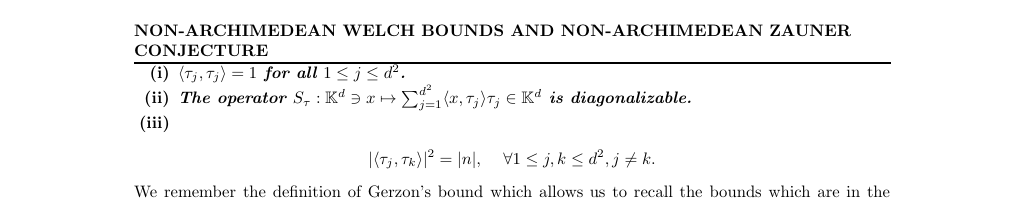
\includegraphics[width=\textwidth]{figures/zauner_conjecture_crop_page5.png}
\end{center}

\section{Proof intuition}

The field hypothesis already collapses the numerical part of every Welch
equality: substituting $r$ copies of $1$ into \eqref{FU} gives $|r|=1$ for
every positive integer $r$.  The source asks only for a \emph{collection} of
vectors and imposes no distinctness or spanning condition.  We may therefore
repeat a single unit vector.  Taking $\tau_j=e_1$ makes every cross inner
product equal to $1$ and makes the frame operator the already diagonal matrix
$\operatorname{diag}(n,0,\ldots,0)$.  Both sides of \eqref{Q-equality} are
then $1$.

\section{Formal result and proof}

\begin{lemma}[Positive integers are units in absolute value]\label{integer-unit}
If $\K$ satisfies \eqref{FU}, then $|r|=1$ for every $r\in\N$.
\end{lemma}

\begin{proof}
In \eqref{FU}, set $\lambda_1=\cdots=\lambda_r=1$.  Then
\[
 |r|=|1^2+\cdots+1^2|=\max_{1\le j\le r}|1|^2=1.
\]
\end{proof}

\begin{theorem}[Complete answer to Question 3.1]\label{main}
Let $\K$ satisfy \eqref{FU}.  For every $d\in\N$ and every $n\ge2$, the
requirements of Question 3.1 are satisfied.  The same holds for $n=1$ under
the natural empty-off-diagonal convention described above.
\end{theorem}

\begin{proof}
Let $e_1=(1,0,\ldots,0)\in\K^d$ and set
\[
 \tau_1=\tau_2=\cdots=\tau_n=e_1.
\]
First, $\langle\tau_j,\tau_j\rangle=\langle e_1,e_1\rangle=1$.
For $x=(x_1,\ldots,x_d)$,
\[
 S_\tau x=\sum_{j=1}^n\langle x,e_1\rangle e_1=nx_1e_1.
\]
Thus the matrix of $S_\tau$ in the standard basis is
$\operatorname{diag}(n,0,\ldots,0)$, so it is diagonalizable (indeed,
already diagonal).  Finally, for every $j\ne k$,
\[
 |\langle\tau_j,\tau_k\rangle|^2=|\langle e_1,e_1\rangle|^2=1.
\]
Lemma \ref{integer-unit} gives $|n|=|d|=1$, hence
\[
 \max_{j\ne k}\{|n|,|\langle\tau_j,\tau_k\rangle|^2\}
 =\max\{1,1\}=1=\frac{1^2}{1}=\frac{|n|^2}{|d|}.
\]
This is precisely the requested equality.
\end{proof}

\begin{corollary}[The stated non-Archimedean Zauner conjecture]\label{zauner}
Conjecture 3.2 holds as written: for every $d\in\N$, take $d^2$ copies of
$e_1$.  For $d\ge2$ all three displayed conditions hold.  For $d=1$, the
off-diagonal universal condition is vacuous.  If the undefined $|n|$ in
condition (iii) is read as either $|d^2|$ or the likely intended $|d|$, its
value is $1$ by Lemma \ref{integer-unit}.
\end{corollary}

\begin{corollary}[Simultaneous equality in every stated Welch order]
For the same repeated collection and every tensor order $m\in\N$, the
higher-order bound of Theorem 2.3 in the source is an equality.
\end{corollary}

\begin{proof}
The induced operator on $\operatorname{Sym}^m(\K^d)$ is $n$ times the
coordinate projection onto $e_1^{\otimes m}$, hence diagonalizable.  Every
cross term has absolute value $1$.  Lemma \ref{integer-unit}, applied also to
the positive integer $\binom{d+m-1}{m}$, makes both sides of the higher-order
bound equal to $1$.
\end{proof}

\section{The stated equiangular-line problem has no finite Gerzon bound}

Question 3.6 asks for a maximum number of vectors satisfying only fixed
self-inner-product and fixed cross-inner-product conditions.  Its statement,
which spans source pages 5--6, is reproduced below.
\begin{center}
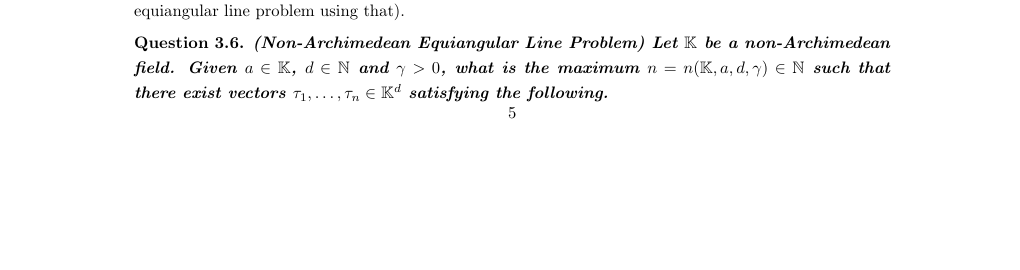
\includegraphics[width=\textwidth]{figures/equiangular_question_crop_page5.png}
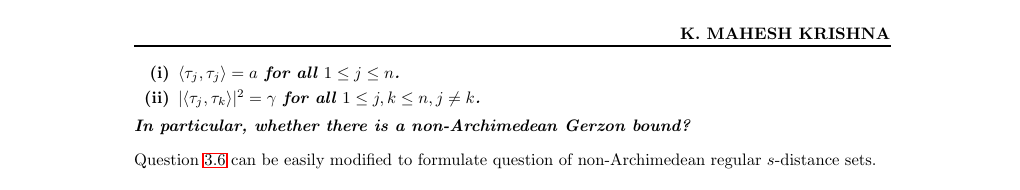
\includegraphics[width=\textwidth]{figures/equiangular_question_crop_page6.png}
\end{center}

\begin{corollary}\label{gerzon}
In the vector formulation of Question 3.6,
$n(\K,1,d,1)$ is unbounded for every $d\in\N$.  Consequently no finite
non-Archimedean Gerzon bound can hold under the displayed hypotheses alone.
\end{corollary}

\begin{proof}
For every prescribed $N\in\N$, take $N$ copies of $e_1$.  Then every
self-inner-product is $1$ and every cross-inner-product has squared absolute
value $1$.  Thus admissible collections exist with arbitrarily large
cardinality.
\end{proof}

\section{Verification notes and limitations}

The argument is purely algebraic and has no numerical or asymptotic
dependency.  The proof audit checked the following points.
\begin{itemize}
 \item Equation \eqref{FU} is quantified over every positive integer, so the
 integer-unit substitution is legitimate for $n$, $d$, and the binomial
 dimensions in the higher-order result.
 \item The source's inner product is bilinear, and $\langle e_1,e_1\rangle=1$.
 \item The displayed frame operator is exactly diagonal in the standard basis.
 \item Neither Question 3.1, Conjecture 3.2, nor the vector conditions in
 Question 3.6 require distinct vectors, distinct one-dimensional subspaces,
 spanning, injectivity, or a tight frame operator.
\end{itemize}

This last point is the essential scope limitation.  If ``Zauner'' or
``equiangular lines'' is strengthened to require $d^2$ distinct lines, or if
$S_\tau$ is required to be a nonzero scalar multiple of the identity, the
repeated-vector construction is inadmissible and this packet makes no claim.
The result is full only for the exact formal statements in the source.

\section{Bounded novelty check and review recommendation}

On 9 August 2026 we searched the run's registry, solution, attempt, and
proof-gap indexes for arXiv:2210.07062 and the core phrases
``Non-Archimedean Zauner Conjecture'', ``Non-Archimedean Welch bounds'', and
``non-Archimedean equiangular line problem''.  We also performed bounded
official-arXiv web searches by exact title, arXiv id, exact conjecture phrase,
``distinct'', and ``solution''.  The source and adjacent classical SIC papers
were found, but no later amendment adding distinctness and no matching
resolution by repeated vectors was located.  Novelty is therefore
provisional and requires expert bibliographic review.

\textbf{Human-review recommendation.}  Verify only two semantic points: that
``collection'' is to be read literally as allowing repetitions, and that the
run evaluates open questions as stated rather than silently importing the
classical distinct-line/tight-frame definition.  Under that literal reading,
the proof is complete.

\enlargethispage{\baselineskip}
\paragraph{Reference.}
[1] K. Mahesh Krishna,
\emph{Non-Archimedean Welch Bounds and Non-Archimedean Zauner Conjecture},
arXiv:2210.07062, 2022,
\url{https://arxiv.org/abs/2210.07062}.

\end{document}
